% Define document class
\documentclass[preprint]{aastex63}
\usepackage{tabularx}
\usepackage{amsmath}

\begin{document}

% Title
\title{Earth's Impact History and the Timing of the Origin of Life}

% Authors
\author{Nicholas F. Wogan}
\affiliation{Department of Earth and Space Sciences, University of Washington, Seattle, WA 98195}
\affiliation{Virtual Planetary Laboratory, University of Washington, Seattle, WA98195}

\author{David C. Catling}
\affiliation{Department of Earth and Space Sciences, University of Washington, Seattle, WA 98195}
\affiliation{Virtual Planetary Laboratory, University of Washington, Seattle, WA98195}

\author{Kevin J. Zahnle}
\affiliation{Space Science Division, NASA Ames Research Center, Moffett Field, CA 94035}
\affiliation{Virtual Planetary Laboratory, University of Washington, Seattle, WA98195}

\begin{abstract}
Big impacts on the early Earth would have created highly reducing atmospheres that generated molecules needed for the origin of life, such as nitriles. However, such impactors can be followed by impactors that were still sufficiently big to vaporize the ocean and destroy any incipient life. In this scenario, a post-impact reducing atmosphere needs to be followed by a lack of subsequent sterilizing impacts for life to persist. Using what we know about the impact history of early Earth and what is needed to generate post-impact highly reducing atmospheres, we show that  the median timing of biopoesis in this impact-driven scenario was $\sim 4.35$ Ga. However, uncertainties are large because impact bombardment is inherently stochastic, so biopoesis could have occurred in $\sim 0.5$ billion year window from 4.45 to 3.9 Ga within 95\% uncertainties of our model. Claims of a far narrower window for the origin of life are unsupported. In our optimistic scenario for life starting from post-impact reducing atmospheres, we find that biopoesis is possible in 92\% of stochastic impact realizations. This potentially bodes well for life on rocky planets elsewhere because they will have experienced an early episode of enhanced impact bombardment given how planets form.
\end{abstract}

\section{Introduction}

\citet{Benner_2020} argued that the most likely time for the origin of life in an RNA-world scenario would have been $4.36 \pm 0.1$ Ga in the wake of a $\sim 2 \times 10^{22}$ kg ($\sim 2100$ km) asteroid impact which they called Moneta. They suggested that iron delivered by Moneta's core would have reacted with impact-vaporized ocean water to generate a reducing Hadean atmosphere conducive to the photochemical generation of essential prebiotic molecules like HCN. This transient period could have been a window of opportunity for the origin of RNA and, ultimately, life.

A single Moneta impact could also explain the highly-siderophile elements (i.e. iron-loving, abbreviated HSEs) in the Moon's and the Earth's mantles. During the moon-forming impact, most all HSEs should have been sequestered in each planetary core, so extant mantle HSEs are commonly interpreted as evidence for late-accretion impactors. Earth's mantle has substantially more HSEs than the Moon by an amount that cannot be accounted for by Earth's greater gravitation cross section \citep{Day_2015}. A single massive Moneta impact could explain the Earth-Moon HSE discrepancy because, by the statistics of small numbers, Moneta could have missed the moon and hit the Earth \citep{Bottke_2010}.

However, the lunar HSE depletion has explanations that do not require a Moneta impact. Lunar HSEs could have been lost to space during impact-delivery because of the Moon's small gravity \citep{Kraus_2015}. Alternatively, HSEs delivered to the Moon during its $\sim 150$ million-year magma ocean could have been sequestered in the core due to iron sulfide exsolution \citep{Morbidelli_2018,Rubie_2016}. Finally, there is some chance that the Earth's HSEs do not record late impacts because the Moon-forming impact delivered HSEs \citep{Sleep_2016}, or because HSEs are gradual core contributions over time from mantle plumes \citep{Halliday_2023,Mundl_2020}. If indeed Earth's HSEs reflect asteroid bombardment after the Moon formed, then the HSEs can be explained by multiple $\sim 500$ to 2000 km impacts rather than a single big ($\sim 2100$ km) collision.

Recently, \citep{Wogan_2023} use photochemical models of post-impact atmospheres to show that impacts significantly smaller than Moneta can efficiently produce prebiotic molecules. In their simulations, impactor iron equilibrates with vaporized ocean water to generate atmospheric H$_2$, and CH$_4$ and NH$_3$ form thermochemically as the reducing steam atmosphere cools. Once steam condense to an ocean, subsequent photochemistry of the Titan-like atmosphere produces prebiotic nitriles. Modeling shows that the production of both HCN and HCCCN only occurs when $\mathrm{CH_4} / \mathrm{CO_2} \gtrsim 0.1$ while the atmosphere is hazy. In an optimistic scenario, which includes nickel catalyzed methane production, modeling suggests that $\mathrm{CH_4} / \mathrm{CO_2} > 0.1$ (i.e. significant nitriles) occurs for impacts $> 4 \times 10^{20}$ kg. In a pessimistic modeling case, which assumes only a fraction of impactor iron reacts with the atmosphere \citep{Citron_2022}, a $> 5 \times 10^{21}$ kg impactor is required to produce substantial HCN and HCCCN. Regardless of uncertainty, \citet{Wogan_2023} show that an impactor much smaller than Moneta could spark an origin of life, and that the \citet{Benner_2020} estimated timing for biopoesis could be inaccurate because it is based on Moneta.

Here, we use the \citet{Wogan_2023} results, along with Monte-Carlo simulations of Earth's impact history to make an alternative estimate for when life most likely emerged during an RNA-first process. Our calculations account for the possibility of planet sterilization by impacts that vaporize the ocean \citep{Sleep_1989}. We assume that a life-starting impact is one that produces significant prebiotic molecules and is not subsequently followed by an ocean-vaporizing impact that destroys the biosphere. By considering the fraction of stochastic impact realizations that do not have an life-starting impact, we also estimate the probability of life beginning if we were to rerun Earth's clock.

\section{Methods} \label{sec:methods}
The rate impacts hit Earth bigger than mass $m$ at age $t$ is given by

\begin{equation}
  f(t,m) = F_0(t) S_0(m)
\end{equation}
Here, $S_0(m)$ is the size-frequency distribution of impactors normalized to a reference mass $m_0$ so that $S_0(m_0) = 1$. Also, $F_0(t)$ is the number of impacts per billion years with mass greater than $m_0$.

We assume the size-frequency distribution of impactors is identical to the main-belt asteroids \citep[Extended Data Figure 1,][]{Marchi_2014}. Data for the frequency of main-belt asteroids only extends down to about 1 km diameter ($1.3 \times 10^{12} $ kg). To extend the distribution to smaller objects, we use the observed 1400 ratio between the frequency of $> 1$ km and $> 20$ km craters on the Moon. \citet{Morbidelli_2018} uses crater scaling relations to show that 1 km and 20 km craters on the Moon corresponds to 50 m and 1 km asteroids, respectively. The largest main belt asteroid is $\sim 1000$ km, so we log-linearly extrapolate to larger impactors (Figure \ref{fig:sfd_and_flux}). Finally, we normalize the size-frequency distribution to the impact mass required to make a 1 km crater on the moon (50 m object, $m_0 = 1.64 \times 10^{8}$ kg). Figure \ref{fig:sfd_and_flux}a shows the resulting size-frequency distribution.

\begin{figure}
  \centering
  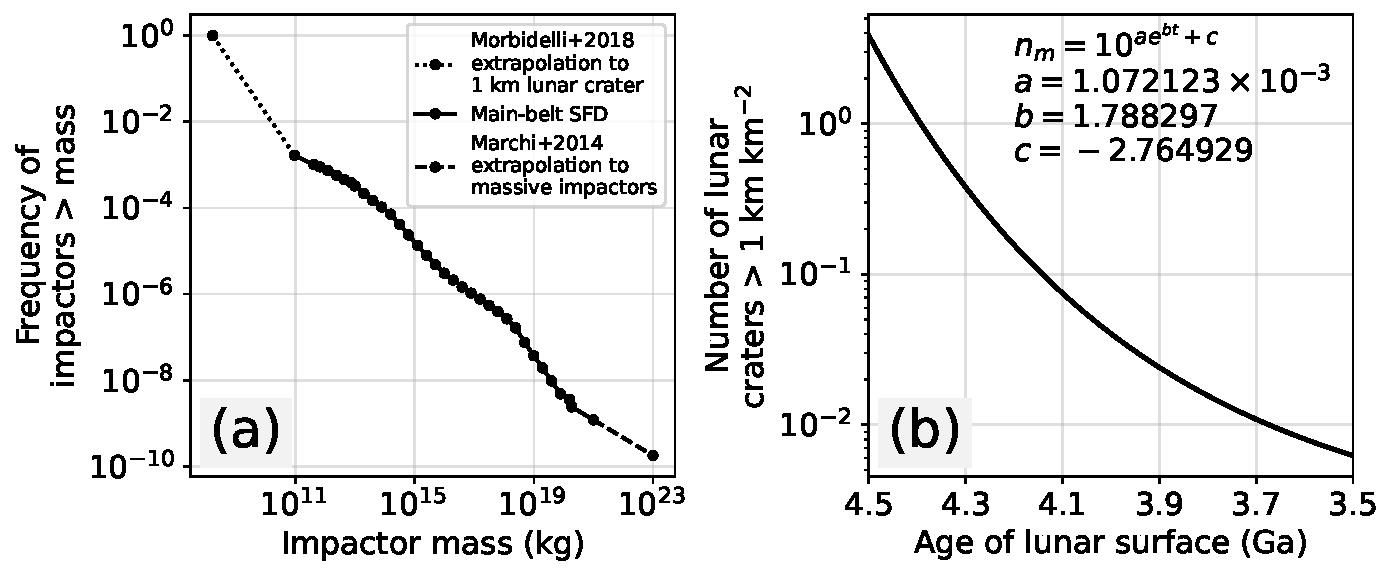
\includegraphics[width=1.0\textwidth]{figures/SFD_and_flux.pdf}
  \caption{Our assumed (a) size-frequency distribution of impactors and (b) lunar cratering record. Most of the size-frequency distribution is identical to the main-belt asteroids \citep[Extended Data Figure 1,][]{Marchi_2014}. We extrapolate to objects $\lesssim 10^{11}$ kg using the observed frequency ratio of $> 1$ km and $> 20$ km lunar craters, and log-linearly extrapolate to asteroids $\gtrsim 10^{21}$ kg. The lunar cratering record is the red line in Figure 5 of \citet{Morbidelli_2018}.}
  \label{fig:sfd_and_flux}
\end{figure}

The flux of impactors, $F_0(t)$, can be estimated from the lunar cratering record. We adopt the accretionary tail scenario discussed in \citet{Morbidelli_2018}. In other words, we assume that the ``late heavy bombardment'' did not happen \citep{Cartwright_2022,Hartmann_2019,Zellner_2017}, and that the impact flux on Earth was constantly decreasing throughout the Hadean eon. Figure \ref{fig:sfd_and_flux}b shows $n_m$, our assumed lunar impact history taken from \citet{Morbidelli_2018} (red line in their Figure 5).

Extrapolating the lunar impact history to Earth requires correcting for Earth's greater gravitational attraction. Assuming the approach velocity of impactors far from the Earth and Moon was on average 18 km/s \citep{Morbidelli_2018}, then Earth should receive $s_0 = 1.36$ times more impacts per surface area than the Moon. Therefore, the number of impacts on Earth is

\begin{equation}
  N_0 = A_\oplus s_0 n_m = A_E s_0 10^{a e^{b t} + c}
  \label{eq:num_earth_impacts}
\end{equation}
Equation \eqref{eq:num_earth_impacts} also accounts for Earth's surface area ($A_\oplus$), making $N_0$ the number of impacts on Earth since age $t$ that cause a crater $> 1$ km on the moon. As discussed previously, \citet{Morbidelli_2018} use crater scaling relations to show that a 1 km lunar crater corresponds to a 50 m object with mass $m_0 = 1.64 \times 10^8$ kg.

The derivative of $N_0$ gives the flux, $F_0$:

\begin{equation}
  F_0(t) = \frac{d N_0}{dt}
\end{equation}
The average number of impacts on Earth between time $t_1$ and $t_2$ with mass greater than $m$ is then

\begin{align}
\begin{split}
  N(m,t_1,t_2) &= \int_{t_1}^{t_2} f(t,m) dt \\
  &= S_0(m) \int_{t_1}^{t_2} \frac{d N_0}{dt} dt \\
  &= S_0(m) A_\oplus s_0 \left( 10^{a e^{b t_2} + c} - 10^{a e^{b t_1} + c} \right)
\end{split}
\end{align}

To simulate impact histories, we consider a fine grid of impactor masses between $10^{12}$ and $10^{23}$ kg, and a grid of times between 4.5 and 3.5 Ga. Indexes $j$ and $i$ indicate the mass and time grid cells respectively, while, for example, $j-\frac{1}{2}$ and $j+\frac{1}{2}$ indicate the edges of the grid cell. We can compute the expected number of impacts within a mass and time grid cell with the following

\begin{equation}
  \overline{N}_{ij} = N(m_{j-\frac{1}{2}},t_{i-\frac{1}{2}},t_{i+\frac{1}{2}}) - N(m_{j+\frac{1}{2}},t_{i-\frac{1}{2}},t_{i+\frac{1}{2}})
\end{equation}
Next, we sample a Poisson distribution for each $\overline{N}_{ij}$, giving a stochastic number of impacts in each mass and time grid cell which constitutes an impact history. Performing this sampling thousands of times captures many of the possible impact histories. We only keep impact histories that accrete a total mass of $2 \times 10^{22}$ and $6 \times 10^{22}$ kg because this is approximately the mass implied by the HSEs in Earth's mantle. This range of masses is based on \citet{Day_2015} who used mantle HSEs to suggest that the Earth was impacted by $\sim 3 \times 10^{22}$ to $4.8 \times 10^{22}$ kg of material, but we choose a wider range of masses because HSEs could have been lost to Earth's core or to space during impacts \citep{Marchi_2018}.

Our final step is to assign impact velocities to each collision in the many sampled impact histories. Appendix Figure \ref{fig:velocity_distribution} shows Earth's impact velocity distribution. We created this distribution using the JPL database of close approaches to Earth by small bodies \citep{Park_2023}, considering all close approach asteroids within 0.05 AU to Earth. The database gives the approach velocity of each asteroid far from Earth, so we compute the impact velocity by accounting for Earth's gravitational energy.

The final collection of sampled impact histories can then be used to compute impact statistics which are relevant to the timing and likelihood of the origin of life.

\section{Results}

\begin{figure}
  \centering
  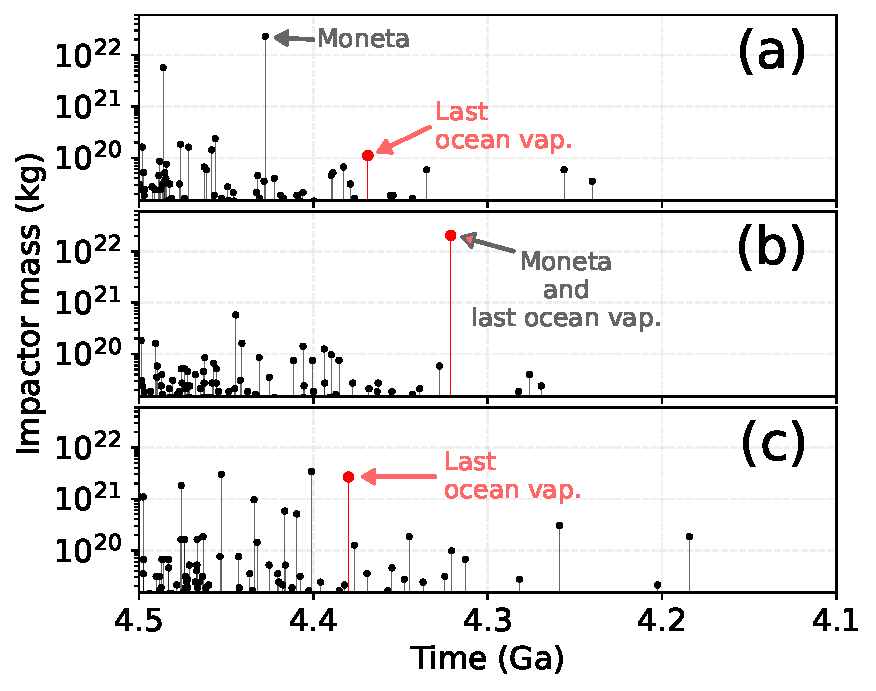
\includegraphics[width=0.65\textwidth]{figures/example_impact_histories.pdf}
  \caption{Three simulated impact histories of the 5000 derived from our Monte-Carlo approach (Section \ref{sec:methods}). Each vertical line indicates an impact of a mass shown by the y-axis.}
  \label{fig:example_impact_histories}
\end{figure}

Figure \ref{fig:example_impact_histories} illustrates three of the 5000 impact histories computed with our Monte-Carlo approach (Section \ref{sec:methods}). In Figure \ref{fig:example_impact_histories}a, a Moneta-sized impact occurs at $\sim 4.43$ Ga delivering nearly all of Earth's mantle HSEs. The impact should also reduce the Hadean atmosphere creating conditions favorable for prebiotic chemistry. However, in this case, Moneta is not a life-starting impact because Moneta is followed by an ocean-vaporizing collision at $\sim 4.37$ Ga which we assume destroys any existing biosphere. Based on smoothed-particle hydrodynamics impact simulations, we nominally assume that 10\% of an impact's kinetic energy goes into vaporizing the ocean \citep[Appendix X,][]{Citron_2022}. Vaporizing the ocean requires $5 \times 10^{27}$ J, so a $> 5 \times 10^{28}$ J impact should deliver sufficient energy. In Figure \ref{fig:example_impact_histories}a, the last ocean-vaporizing impact is only $\sim 10^{20}$ kg (360 km) but has a large impact velocity of $32$ km/s giving it $5.12 \times 10^{28}$ J of kinetic energy. 

Moneta also occurs in the Figure \ref{fig:example_impact_histories}b impact realization. In this scenario, any life created in the wake of Moneta should not be subsequently exterminated because Moneta is the last impact to vaporize the ocean.

Figure \ref{fig:example_impact_histories}c shows a impact history where Moneta does not occur. Instead, Earth's mantle HSEs are delivered by multiple $10^{21}$ to $4 \times 10^{21}$ kg collisions. Whether this bombardment history would cause biopoesis depends on the required minimum impact mass to produce significant origin of life molecules. \citet{Wogan_2023} uses photochemical models of post-impact atmospheres to show that, optimistically, an impact $> 4 \times 10^{20}$ kg should give rise to an atmosphere that makes significant prebiotic molecules. Under this optimistic requirement, the last ocean-vaporizing impact in Figure \ref{fig:example_impact_histories}c at 4.38 Ga with mass $3 \times 10^{21}$ kg could successfully start life. However, with pessimistic modeling assumptions, \citet{Wogan_2023} finds that a $> 5 \times 10^{21}$ kg impact is instead required for biopoesis. In this alternative scenario, an origin of life never occurs in Figure \ref{fig:example_impact_histories}c because there is no impact larger than $5 \times 10^{21}$ kg.

\begin{figure}
  \centering
  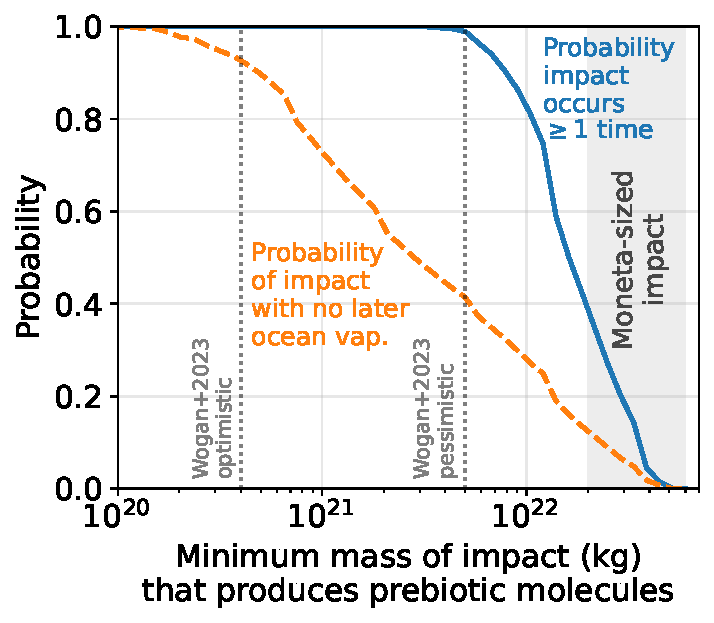
\includegraphics[width=0.5\textwidth]{figures/probabilities_of_impacts.pdf}
  \caption{The probability of an impact-driven origin of life on Earth. The blue solid line is the probability of an impact occurring at least once. The orange dashed line is the probability of an impact without a subsequent ocean-vaporizing collision, which can be interpreted as the chance of an impact that starts life. Probabilities are shown as a function of the minimum impact mass to produce significant prebiotic molecules. Two plausible minimum masses are the \citet{Wogan_2023} optimistic and pessimistic scenarios indicated with vertical dotted lines. The shaded region between $2 \times 10^{22}$ and $6 \times 10^{22}$ kg are Moneta-sized impacts because they deliver most all of Earth's mantle HSEs. There is a 92\% chance of a life-starting impact in the \citet{Wogan_2023} optimistic case, and a 41\% chance in the pessimistic case.}
  \label{fig:probabilities_of_impacts}
\end{figure}

As illustrated in Figure \ref{fig:example_impact_histories}, a life-starting impact does not occur in every simulated impact history. In our impact-driven model for the origin of life, biopoesis requires (1) an impact of sufficient mass to make prebiotic molecules and (2) the lack of a later ocean-vaporizing collision that destroys the biosphere without rekindling it. Figure \ref{fig:probabilities_of_impacts} shows the probability of conditions (1) and (2) occurring as a function of the minimum impact mass that produces prebiotic molecules. For example, consider the \citet{Wogan_2023} optimistic minimum mass of $4 \times 10^{20}$ kg indicated in Figure \ref{fig:probabilities_of_impacts}. All simulated impact histories have at least one impact bigger than $4 \times 10^{20}$ kg (blue line in Figure \ref{fig:probabilities_of_impacts}). However, the probability of the origin of life in this scenario is 92\%, because 8\% of the time the last $4 \times 10^{20}$ kg collision is followed by a smaller ocean-vaporizing impact that perhaps sterilizes the planet (orange dashed line in Figure \ref{fig:probabilities_of_impacts}). An origin of life is less probable if we consider the \citet{Wogan_2023} pessimistic minimum mass ($> 5 \times 10^{21}$ kg) to produce significant origin of life molecules. A $> 5 \times 10^{21}$ kg impact without later ocean vaporization occurs only 41\% of the time.

\begin{figure}
  \centering
  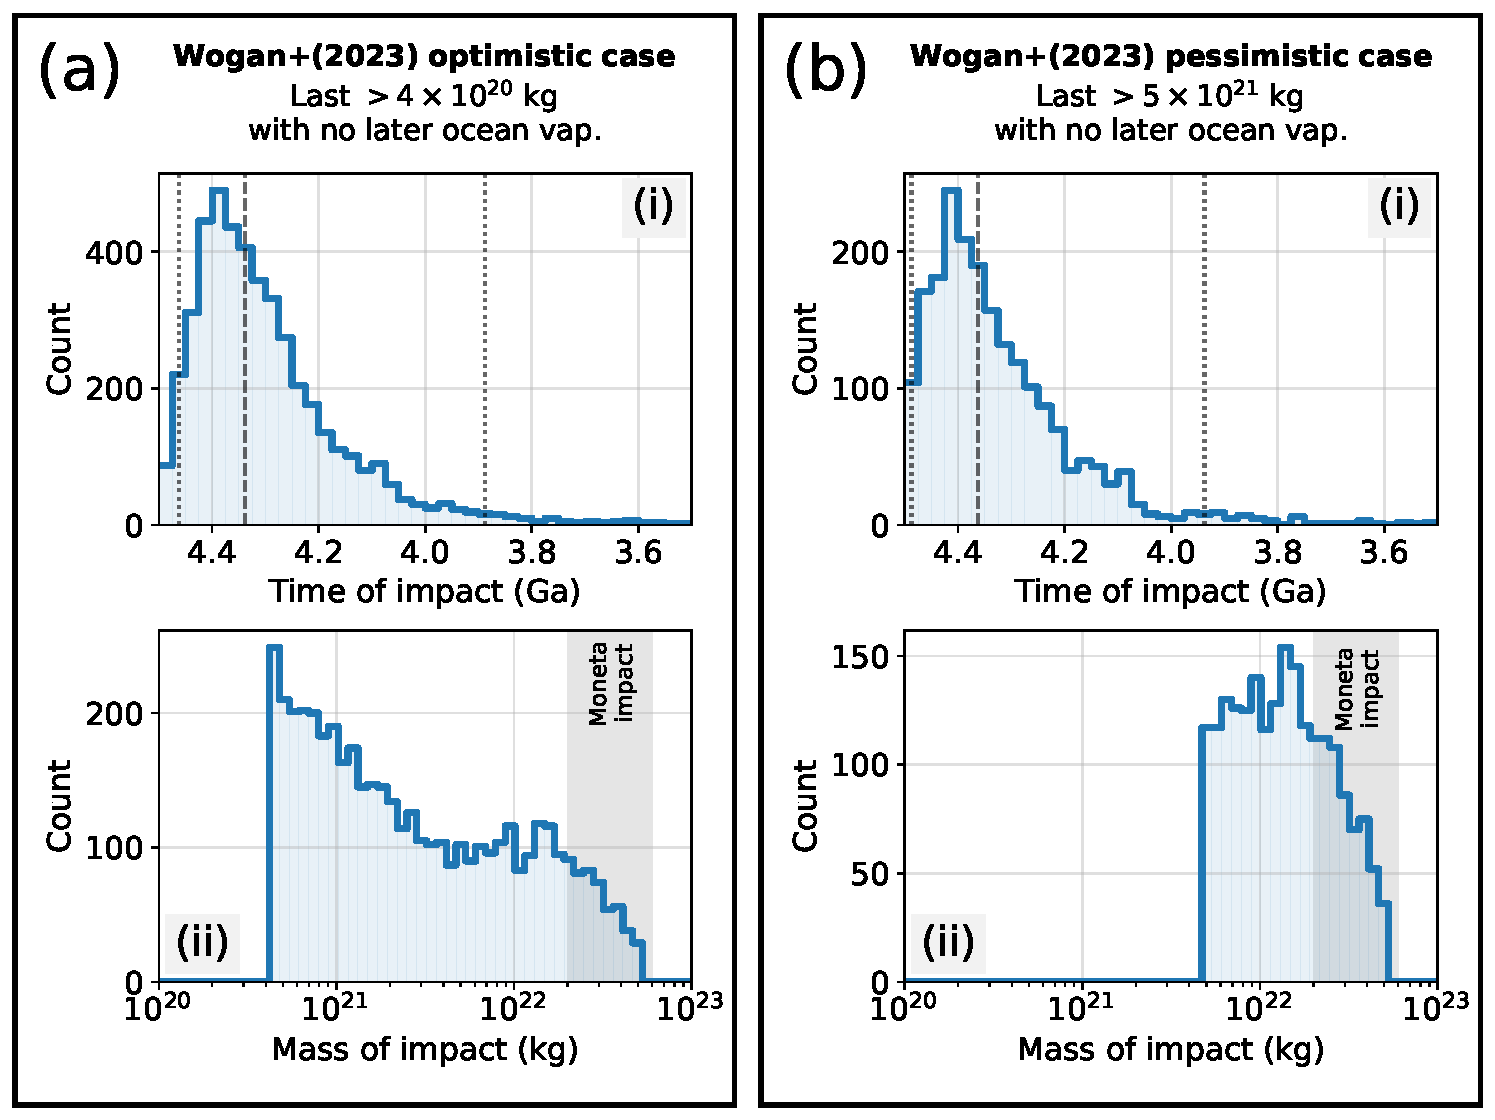
\includegraphics[width=0.85\textwidth]{figures/timing_and_mass.pdf}
  \caption{The timing and mass of a life-starting impact on the early Earth. (a) considers an optimistic minimum impact mass needed to generate the molecules for an RNA origin of life and (b) examines a pessimistic minimum impact mass \citep{Wogan_2023}. In either (a) or (b), panels (i) and (ii) show probability distributions for the timing and mass, respectively, of the last impact the produces prebiotic molecules which does not have a later ocean-vaporizing collision. The vertical dashed lines on (a) i and (b) i plot are median values, and the vertical dotted lines are the 95\% confidence intervals. In an impact-driven origin of life, biopoesis most likely occurred $\sim 4.35$ Ga with a 95\% uncertainty between approximately 3.9 and 4.45 Ga.}
  \label{fig:time_and_mass}
\end{figure}

To estimate the most likely timing for the origin of life, we consider both the \citet{Wogan_2023} optimistic and pessimistic criteria. Figure \ref{fig:time_and_mass}a is the optimistic case, showing the timing (Figure \ref{fig:time_and_mass}a (i)) and mass (Figure \ref{fig:time_and_mass}a (ii)) of the last $> 4 \times 10^{20}$ kg impact for the 92\% of impact histories that do not experience later ocean vaporization. The median timing of a life-starting impact is 4.34 Ga with 95\% uncertainty between 3.89 and 4.46 Ga. The large uncertainty mostly stems from the stochastic, Poisson nature of asteroid bombardment. The probability distribution for the mass of the life-starting impact peaks at $4 \times 10^{20}$ kg and decreases with increasing mass because of the size-frequency distribution of asteroids (Figure \ref{fig:sfd_and_flux}a). There is only a 10\% chance that the impact is Moneta-sized (i.e., between $2 \times 10^{22}$ and $6 \times 10^{22}$ kg).

The timing of an origin of life impact is qualitatively unchanged when instead adopting the \citet{Wogan_2023} pessimistic case, which requires a $> 5 \times 10^{21}$ kg impact without later ocean vaporization (Figure \ref{fig:time_and_mass}b). In this scenario, the median timing for life's origin is 4.36 Ga with a 95\% confidence interval spanning 3.94 to 4.49 Ga (Figure \ref{fig:time_and_mass}b (i)). Under these assumptions, the life-starting impact is Moneta-sized 31\% of the time (Figure \ref{fig:time_and_mass}b (ii)), which is more probable compared to ``optimistic'' case (Figure \ref{fig:time_and_mass}a (ii)).

\section{Discussion and Conclusions}

We use Monte-Carlo simulations of Earth's impact history to determine the most likely timing for the origin of life in an RNA-first processes. We make use of results of \citep{Wogan_2023}, who find that significant origin of life molecules, such as HCN, are produced in the Hadean atmosphere after a $> 4 \times 10^{20}$ kg impact in an optimistic case, and after a $> 5 \times 10^{21}$ kg impact in a pessimistic scenario. We consider both possibilities, and assume such impacts can cause life's origin so long as they are not followed by a smaller ocean-vaporizing collision that sterilizes the planet.

For either the optimistic or pessimistic cases, we find that the most likely timing for an origin of life impactor is $\sim 4.35$ Ga with a 95\% uncertainty spanning the entire Hadean eon (approximately 4.45 to 3.9 Ga). The large uncertainty is caused by the intrinsic stochastic nature of impacts. These results suggest that the \citet{Benner_2020} proposed timing of the origin of life, at $4.36 \pm 0.1$ Ga, is too narrow. Furthermore, the mass of the life starting impactor is most likely (69\% to 90\% probability) smaller than the Moneta impactor (Figure \ref{fig:time_and_mass}) proposed by \citet{Benner_2020}, because the size frequency distribution of asteroids prefers more frequent smaller impactors.

% Caveats
% While the modeling effort described above attempts to use the most current understanding of Earth's impact history and its effects,

Our simulations of Earth's impact history do not always result in an origin of life. There are some impact histories where a collision of sufficient mass to produce prebiotic molecules does not occur, or alternatively, does occur but primitive life is subsequently destroyed by an ocean-vaporizing impact that does not rekindle the biosphere. A life-starting impact occurs 92\% or 41\% of the time when we assume a $> 4 \times 10^{20}$ kg or $> 5 \times 10^{21}$ kg impact without later ocean-vaporization is required to start life, respectively. 

If life began in an RNA process after an impact, then this work suggests that origin of life on Earth was not an anomalous event and was indeed strongly favored (92\% chance) under optimistic assumptions. Given that rocky exoplanets accreted from impacts, our work supports and optimistic outlook for life on exoplanets and future searches for biosignatures. 

\section*{Acknowledgements}

N.F.W. and D.C.C. were supported by the Simon's Collaboration on Origin of Life Grant 511570 (to D.C.C.). Also, N.F.W., D.C.C., and K.J.Z. were supported by NASA Astrobiology Program Grant 80NSSC18K0829 and benefited from participation in the NASA Nexus for Exoplanet Systems Science research coordination network. N.F.W. and D.C.C. also acknowledge support from Sloan Foundation Grant G-2021-14194. K.J.Z. was supported by NASA Exobiology Grant 80NSSC18K1082.

\appendix

\renewcommand{\thefigure}{A\arabic{figure}}
\renewcommand{\thetable}{A\arabic{table}}
\setcounter{figure}{0}
\setcounter{table}{0}

\begin{figure}
  \centering
  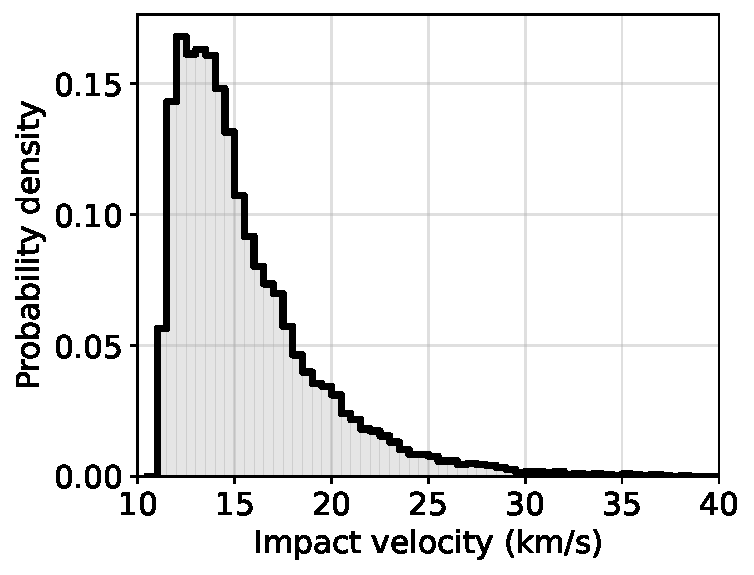
\includegraphics[width=0.4\textwidth]{figures/velocity_distribution.pdf}
  \caption{Our assumed probability distribution for the velocity of impacts derived from modern observations of asteroid close approaches \citep{Park_2023}.}
  \label{fig:velocity_distribution}
\end{figure}


\bibliography{bib}
\bibliographystyle{aasjournal}

\end{document}
